\chapter{Coupled Cluster}
\label{ch:impl_coupled_cluster}

The main product of this study is manifested in the \lstinline{coupled_cluster}
module for Python. This module is designed to fit together with the
\lstinline{quantum_systems} module described in the previous chapter. We have tried to 
make this module easy to extend, resulting in a framework where every solver scheme 
inherits from an abstract parent class that specifies what must be implemented in order 
to make a supplemental solver class operational in conjunction with the rest of the 
framework.

As a beginning to this project, which we hope will continue to grow and be used, 
we have implemented several different ground state solver classes, and several
time-dependent solver classes. In order of increasing sophistication and 
elegance, we have a ground state- and a time-dependent solver for both the coupled cluster
method
with double excitations (CCD), the coupled cluster method with singles- and double 
excitations (CCSD), and for the orbital-adaptive coupled cluster method with double
excitations (OACCD). The time-dependent solvers within a particular category are 
dependent on its ground state counterpart, but the ground state solvers can be used
independently.

A complete diagrammatic class hierarchy of the \lstinline{coupled_cluster} module 
can be found in \autoref{fig:class_diagram_coupled_cluster}. This class hierarchy also illustrates how 
the \lstinline{coupled_cluster} module fits into and works with the 
\lstinline{quantum_systems} module. This figure is the same figure as the one shown in 
\autoref{fig:class_diagram_quantum_systems}, but inserting the class diagram 
here as well should make this chapter easier to read.

\begin{figure}
    \centering
    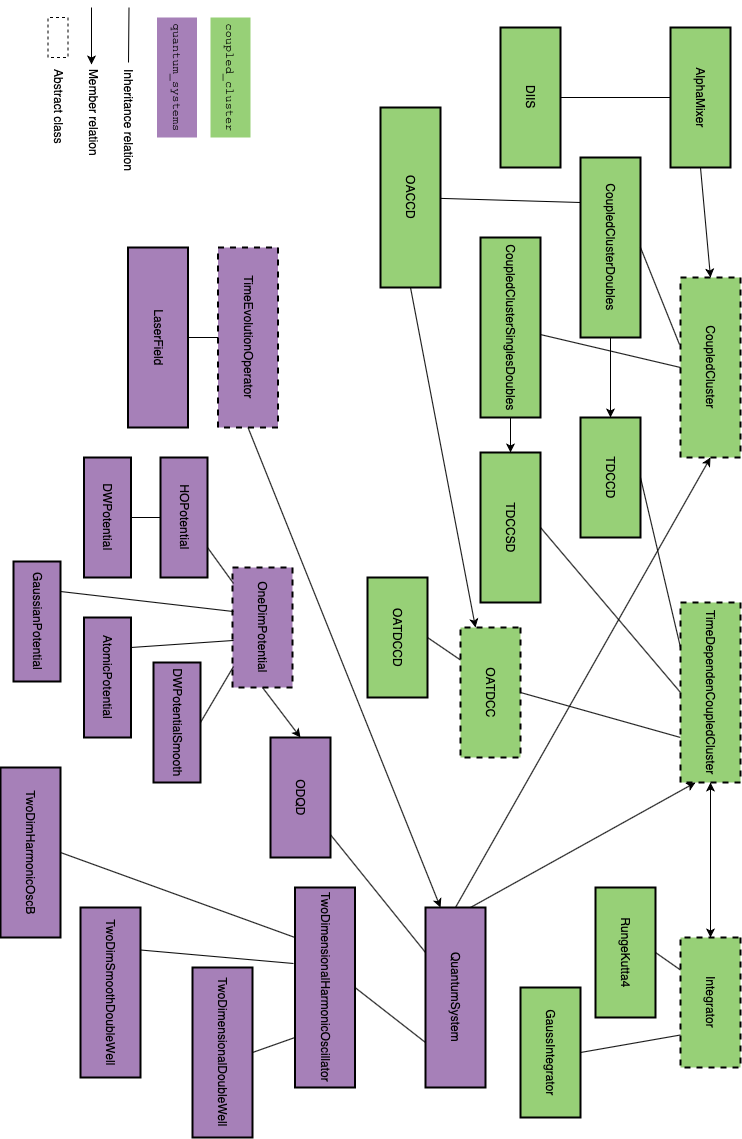
\includegraphics[width=\textwidth]{implementation/figures/taifun_class_diagram.png}
    \caption{Class hierarchy of the two Python modules, \lstinline{coupled_cluster}
    and \lstinline{quantum_systems}.}
    \label{fig:class_diagram_coupled_cluster}
\end{figure}

The \lstinline{coupled_cluster} module can be installed from github via \lstinline{pip}
by the following command,
\begin{lstlisting}[language=bash]
pip install git+https://github.com/Schoyen/coupled-cluster.git
\end{lstlisting}
If one prefers, the same task can be accomplished by the following commands,
\begin{lstlisting}[language=bash]
git clone https://github.com/Schoyen/coupled-cluster.git
cd coupled-cluster
pip install .
\end{lstlisting}
We have supplied environment specifications for \lstinline{conda}, with requirement 
specifications for the convenience of the user. Assuming the git repository is cloned 
properly,
\begin{lstlisting}[language=bash]
conda environment create -f environment.yml
\end{lstlisting}
Activate the environment with,
\begin{lstlisting}[language=bash]
conda activate cc
\end{lstlisting}
Full documentation of this module, which we hope will be kept up to date with any future revisions 
can be found at \url{www.coupled-cluster.com}.

\section{Ground State Computations}

    Before any development in time can be performed, we need to arrive at configurations 
    of systems that 
    we can be somewhat certain exist in nature. This makes the implementation of ground 
    state solvers necessary. We have implemented several ground state solvers; the
    \lstinline{CoupledClusterDoubles} and \lstinline{CoupledClusterSinglesDoubles} 
    are based on the theoretical framework from the Lagrangian formulation of Coupled 
    Cluster theory (see \autoref{sec:lagrangian_cc}),
    while \lstinline{OATDCCD} is a ground state version of an orbital-adaptive 
    ground state coupled cluster solver with double excitations. Moreover, we constructed 
    a data structure for the amplitudes in the \lstinline{AmplitudeContainer} class and 
    we have implemented two ``mixer'' classes that help with convergences of the ground
    state solvers, \lstinline{AlphaMixer} and \lstinline{DIIS}.

    \begin{figure}[h]
    \begin{tcolorbox}
    {\fontfamily{cmss}\selectfont
    \textbf{class} coupled\_cluster.cc\_helper.\textbf{AmplitudeContainer}
    (\emph{t}, \emph{l}, \emph{np})

    \vspace{1em}
    Container for amplitude functions.

    \vspace{1em}
    \textbf{Parameters:}

    \hspace{2em}\textbf{t}(\emph{list}, \emph{tuple}, \emph{set}) $\tau$ amplitudes

    \hspace{2em}\textbf{l}(\emph{list}, \emph{tuple}, \emph{set}) $\lambda$ amplitudes

    \hspace{2em}\textbf{np}(\emph{module}) Matrix library, e.g. numpy, cupy etc

    \vspace{1em}
    \textbf{Attributes:}

    \hspace{2em} \textbf{t} $\tau$ amplitudes

    \hspace{2em} \textbf{l} $\lambda$ amplitudes

    \vspace{1em}
    \textbf{Methods:}

    \hspace{2em} \textbf{unpack}()
    \begin{adjustwidth}{4em}{}
        \textbf{Returns:} Amplitudes

        \textbf{Return type:} \emph{generator}
    \end{adjustwidth}

    \hspace{2em} \textbf{asarray}()
    \begin{adjustwidth}{4em}{}
        \textbf{Returns:} Amplitude vector

        \textbf{Return type:} \emph{np.array}
    \end{adjustwidth}

    }
\end{tcolorbox}
    \end{figure}

    \subsection{Representation of Amplitudes}

    The most central structure in any Coupled Cluster solver the way we represent
    the amplitudes. The 
    amplitudes are what define the true structure of the wavefunction as a linear 
    combination of single-particle functions contained in the reference state Slater 
    determinant. We have found it beneficial to implement a special container 
    class for the amplitudes, aptly called \lstinline{AmplitudeContainer}.

    The \lstinline{AmplitudeContainer} class is built as a data structure for 
    the amplitude functions, and comprises all methods and attributes to serve this 
    purpose. This includes overloading of primitive methods of the base 
    python \lstinline{Object} type.: \lstinline{__add__} and \lstinline{__radd__}
    enables adding a scalar or properly shaped vector to the amplitudes, 
    \lstinline{__mul__} and \lstinline{__rmul__} allows for multiplication 
    with scalars and vectors, and \lstinline{__iter__} is implemented to make 
    the class an iterable. In summary, the \lstinline{AmplitudeContainer} 
    functions as a fully operational data structure for amplitudes of coupled 
    cluster solver, with both $\tau$ and $\lambda$ amplitudes. The $\tau$-amplitudes
    are first introduced in \ref{sec:cluster_operator} and the $\lambda$-amplitudes 
    are introduced in \ref{sec:lagrangian_cc}. 

    \subsection{Coupled Cluster Base Class}

    \begin{figure}
    \begin{tcolorbox}
    {\fontfamily{cmss}\selectfont
    \textbf{class} coupled\_cluster.cc.\textbf{CoupledCluster}

    \hspace{1em}(\emph{system}, \emph{mixer=<class'coupled\_cluster.mix.DIIS'>}, 
        \emph{verbose=False}, \emph{np=None})

    \vspace{1em}
    Abstract base class defining the basic structure of a coupled cluster ground state 
    solver class.
    
    \vspace{1em}
    \textbf{Parameters}

    \hspace{2em}\textbf{system}(\emph{QuantumSystem}) A system class from the 
        \emph{quantum\_systems} module.

    \hspace{2em}\textbf{mixer}(\emph{AlphaMixer, default AlphaMixer}) Mixer - 
        Subclass of \emph{AlphaMixer} class.

    \hspace{2em}\textbf{verbose}(\emph{bool, default False}) Will print results 
        for each iteration if \emph{True}.

    \vspace{1em}
    \textbf{Methods}

    \hspace{2em} \textbf{compute\_ground\_state}
        (\emph{t\_args=[]}, \emph{t\_kwargs=\{\}}, \emph{l\_argys=[]}, \emph{l\_kwargs=\{\}})
        \begin{adjustwidth}{4em}{}
        Computes ground state of system given as parameter. Allows for parameters relating 
        the the $\tau$- and $\lambda$ amplitudes, for use in inheriting classes.
        \end{adjustwidth}
    
    \hspace{2em} \textbf{compute\_particle\_density}()
        \begin{adjustwidth}{4em}{}
        Computes the one-body density of the system.
   
        \textbf{Returns:} Particle density 
  
        \textbf{Return type:} \emph{np.array}
        \end{adjustwidth}
    
    \hspace{2em} \textbf{compute\_reference\_energy}()
        \begin{adjustwidth}{4em}{}
        Computes reference energy

        \textbf{Returns:} Reference energy

        \textbf{Return type:} \emph{np.array}
        \end{adjustwidth}
    
    \hspace{2em} \textbf{get\_amplitudes}(\emph{get\_t\_0=False})
        \begin{adjustwidth}{4em}{}
        Getter for amplitudes.

        \textbf{Parameters:} 
        
            \hspace{1.5em} \textbf{get\_t\_0} (\emph{bool, default False}) 
            Returns amplitude at $t=0$ if \lstinline{True}.

        \textbf{Returns:} Amplitudes

        \textbf{Return type:} \emph{AmplitudeContainer}

        \end{adjustwidth}

    \hspace{2em} \textbf{iterate\_l\_amplitudes} 
        (\emph{max\_iterations=$100$}, \emph{tol=$1e^{-4}$}, \emph{**mixer\_kwargs})
        \begin{adjustwidth}{4em}{}
            Finds solution to $\lambda$ amplitudes iteratively.

        \textbf{Parameters:} 
        
        \hspace{1.5em} \textbf{max\_iterations} (\emph{int})
            The limit of iterations allowed.

        \hspace{1.5em} \textbf{tol} (\emph{float, default $1e^{-4}$})
            The tolerance for convergence.

        \end{adjustwidth}
 
    \hspace{2em} \textbf{iterate\_t\_amplitudes} 
        (\emph{max\_iterations=$100$}, \emph{tol=$1e^{-4}$}, \emph{**mixer\_kwargs})
        \begin{adjustwidth}{4em}{}
            Finds solution to $\tau$ amplitudes iteratively.

        \textbf{Parameters:} 
        
        \hspace{1.5em} \textbf{max\_iterations} (\emph{int})
            The limit of iterations allowed.

        \hspace{1.5em} \textbf{tol} (\emph{float, default $1e^{-4}$})
            The tolerance for convergence.

        \end{adjustwidth}
        
    \hspace{2em} \textbf{\_get\_t\_copy} Abstract method

    \hspace{2em} \textbf{\_get\_l\_copy} Abstract method

    \hspace{2em} \textbf{compute\_energy} Abstract method

    \hspace{2em} \textbf{compute\_one\_body\_density\_matrix} Abstract method

    \hspace{2em} \textbf{compute\_t\_amplitudes} Abstract method

    \hspace{2em} \textbf{compute\_l\_amplitudes} Abstract method

    \hspace{2em} \textbf{setup\_t\_mixer} Abstract method

    \hspace{2em} \textbf{setup\_l\_mixer} Abstract method

    \hspace{2em} \textbf{compute\_t\_residuals} Abstract method

    \hspace{2em} \textbf{compute\_l\_residuals} Abstract method

    }
\end{tcolorbox}
    \end{figure}

    All ground state solvers within the \lstinline{coupled_cluster} module are built 
    as sub-classes of the abstract base class \lstinline{CoupledCluster}. The most
    important method of this class is the \lstinline{compute_ground_state()} method.
    This method in turn calls the \lstinline{iterate_t_amplitudes()} and 
    \lstinline{iterate_l_amplitudes()} successively. 

    As we have outlined in 
    \autoref{ch:coupled_cluster_theory}, the $\tau$ amplitudes are only dependent on 
    $\tau$, while the $\lambda$ amplitudes are dependent on both $\tau$ and $\lambda$.
    Therefore, the $\tau$ amplitude equations iterative solver
    \lstinline{iterate_t_amplitudes()} is called first, and the $\lambda$ amplitude
    equation solver is called second.
    For illustration, the most important section of the \lstinline{compute_l_amplitudes()} method 
    is the following
    \begin{python}
    for i in range(max_iterations):
    self.compute_l_amplitudes()
    residuals = self.compute_l_residuals()

    if self.verbose:
        print(f"Iteration: {i}\tResiduals (l): {residuals}")

    if all(res < tol for res in residuals):
        break

    assert i < (
        max_iterations - 1
    ), f"The l amplitudes did not converge. Last residual: {residuals}" 
    \end{python}
    The equivalent section of code in the \lstinline{compute_t_amplitudes()} method is 
    nearly identical.
    The \lstinline{CoupledCluster} class is supposed to provide a framework for which 
    to implement various coupled cluster ground state solver classes. It therefore
    has several abstract methods that such subclasses need to implement and overwrite.
    The most important of these are the methods \lstinline{compute_t_amplitudes} 
    and \lstinline{compute_l_amplitudes}, which are supposed to contain the evaluation 
    of amplitude equations for a given coupled cluster truncation and scheme. 

    With the hope that the functionality of the rest of the methods 
    in the abstract base class \lstinline{CoupledCluster} can be inferred from 
    name, and with the goal of brevity we proceed to a study of the simplest 
    ground state coupled cluster solver, namely CCD, implemented in the 
    \lstinline{CoupledClusterDoubles} class. 

    \subsection{Coupled Cluster Doubles}

    \begin{figure}
    \begin{tcolorbox}
    {\fontfamily{cmss}\selectfont
    \textbf{class} coupled\_cluster.cc.\textbf{CoupledClusterDoubles}
    (\emph{system}, \emph{**kwargs})

    \vspace{1em}
    Implementation of coupled cluster with double excitations ground state solver. 
    Inherits from the \textbf{CoupledCluster} abstract base class.

    \vspace{1em}
    \textbf{Parameters}

    \hspace{2em}\textbf{system}(\emph{QuantumSystem}) A system class from the 
        \emph{quantum\_systems} module.

    \vspace{1em}
    \textbf{Methods} 
 
    \hspace{2em} \textbf{compute\_ground\_state}
        (\emph{t\_args=[]}, \emph{t\_kwargs=\{\}}, \emph{l\_args=[]}, \emph{l\_kwargs=\{\}})
        \begin{adjustwidth}{4em}{}
        Computes CCD ground state of given system.
        \end{adjustwidth}  

    \hspace{2em} \textbf{compute\_initial\_guess}()
        Computes initial guess for amplitudes.
        %\begin{adjustwidth}{4em}{}
        %\end{adjustwidth}

    \hspace{2em} \textbf{\_get\_t\_copy}()
        \begin{adjustwidth}{4em}{}
        \textbf{Returns:} Copy of $\tau^{ab}_{ij}$ amplitudes
        
        \textbf{Return type:} \emph{AmplitudeContainer}
        \end{adjustwidth}

    \hspace{2em} \textbf{\_get\_l\_copy}()
        \begin{adjustwidth}{4em}{}
        \textbf{Returns:} Copy of $\lambda^{ij}_{ab}$ amplitudes
        
        \textbf{Return type:} \emph{AmplitudeContainer}
        \end{adjustwidth}

    \hspace{2em} \textbf{compute\_t\_residuals}()
        \begin{adjustwidth}{4em}{}
        \textbf{Returns:} Norm of $\tau^{ab}_{ij}$ amplitudes
        
        \textbf{Return type:} \emph{float}
        \end{adjustwidth}

    \hspace{2em} \textbf{compute\_l\_residuals}()
        \begin{adjustwidth}{4em}{}
        \textbf{Returns:} Norm of $\lambda^{ij}_{ab}$ amplitudes
        
        \textbf{Return type:} \emph{float}
        \end{adjustwidth}

    \hspace{2em} \textbf{setup\_t\_mixer}(\emph{**kwargs})
        Sets up mixer for $\tau$ amplitudes

    \hspace{2em} \textbf{setup\_l\_mixer}(\emph{**kwargs})
        Sets up mixer for $\lambda$ amplitudes

    \hspace{2em} \textbf{compute\_energy}()
        \begin{adjustwidth}{4em}{}
        \textbf{Returns:} CCD ground state energy

        \textbf{Return type:} {\emph{float}}
        \end{adjustwidth}

    \hspace{2em} \textbf{compute\_t\_amplitudes}()
        Computes $\tau$ amplitudes

    \hspace{2em} \textbf{compute\_l\_amplitudes}()
        Computes $\lambda$ amplitudes
    
    \hspace{2em} \textbf{compute\_one\_body\_density}()
        \begin{adjustwidth}{4em}{}
        \textbf{Returns:} One-body density matrix

        \textbf{Return type:} \emph{np.array}
        \end{adjustwidth}

    \hspace{2em} \textbf{compute\_two\_body\_density}()
        \begin{adjustwidth}{4em}{}
        \textbf{Returns:} Two-body density matrix

        \textbf{Return type:} \emph{np.array}
        \end{adjustwidth}

    }
\end{tcolorbox}
    \end{figure}
    
    Starting from construction, the \lstinline{CoupledClusterDoubles} class passes 
    the system, defined through a \lstinline{QuantumSystem} object to the 
    parent class constructor, along with any keyword arguments, such as turning 
    on verbosity, mixer type and what matrix library to apply. The
    \lstinline{QuantumSystem} class will contain all the information necessary to 
    set up the system, i.e. construct a one-body matrix, fock matrix and two-body 
    matrix. These will be used to set up empty arrays for the $\tau$ and $\lambda$ 
    amplitudes. The \lstinline{compute_initial_guess} is called lastly in the 
    constructor, computing the inital guess of the double-excited amplitudes as 
    \begin{equation}
        \label{eq:ccd_inital_guess}
        \tau^{(0)} = \frac{u^{ab}_{ij}}{D^{ab}_{ij}},
    \end{equation}
    where $u$ is the two-body operator and
    $D^{ab}_{ij} = f^a_a + f^b_b - f^i_i - f^j_j$,
    where $f$ is the Fock operator.
    
    In the \lstinline{CoupledClusterDobles} class specification one would
    notice that it has implementations of all the abstract methods 
    from the \lstinline{CoupledCluster} abstract class. The reason for the existence 
    of the class, the \lstinline{compute_ground_state()} method, is inherited from the 
    parent class, and does the same thing as described above - calling 
    \lstinline{iterate_t_amplitudes()} and \lstinline{iterate_l_amplitudes()}. These 
    methods also exist as members of \lstinline{CoupledClusterDoubles}, but are excluded 
    from the class specification for sake of brevity. It is 
    possible to pass arguments to the the two iterator methods; one list for each iteration
    method, or as keywords.
    One can also pass arguments 
    to the mixer through the \lstinline{compute_ground_state_method()}. 
    An overview of mixing applied to iterative solvers is given in the next 
    section.

    The important part of the specific coupled cluster scheme solver is contained in the two 
    methods \lstinline{compute_t_amplitudes()} and \lstinline{compute_l_amplitudes()}.
    These functions evaluate the entire coupled cluster doubles amplitude equations.
    The computation of each term (diagram) in the amplitude equation is done in separate functions,
    as calls to \lstinline{numpy.tensordot()}, for a total of ten terms for the 
    $\tau$ amplitude equation in the coupled cluster doubles method including 
    permutation operators:
    \begin{equation}
        \label{eq:ccd_tau}
        \begin{aligned}
        0 =& u^{ab}_{ij} + f^b_c \tau^{ac}_{ij}P(ab) 
            - f^k_j \tau^{ab}_{ik}P(ij)
            + \frac{1}{4} \tau^{ac}_{ij} \tau^{ab}_{mn}u^{mn}_{cd} 
            + \frac{1}{2} \tau^{cd}_{ij}u^{ab}_{cd}
            + \frac{1}{2} \tau^{cd}_{jm} \tau^{ab}_{in} u^{mn}_{cd}P(ij) \\
            &\ - \frac{1}{2} \tau^{ac}_{nm} \tau^{bd}_{ij} u^{nm}_{cd}P(ab)
            + \tau^{ac}_{im} \tau^{bd}_{jn}u^{mn}_{cd}P(ij)
            + \tau^{ac}_{im}u^{bm}_{jc}P(ab)P(ij)
            + \frac{1}{2} \tau^{ab}_{mn}u^{mn}_{ij}.
        \end{aligned}
    \end{equation}

    The initial guess in equation \autoref{eq:ccd_inital_guess} is terms 2 and 3
    from \autoref{eq:ccd_tau}. These terms also form the basis of the iterative scheme,
    if we move them to the left of the equal sign in \autoref{eq:ccd_tau}, 
    \begin{equation}
        D^{ab}_{ij} \tau^{ab}_{ij} = g(u, \tau),
    \end{equation}
    where $g(u, \tau)$ now consists of the rest of the doubles amplitude equation, our 
    recursion relation can be written
    \begin{equation}
        t^{(k+1)} = \frac{g(u,\tau^{(k)})}{D^{ab}_{ij}}.
    \end{equation}

    An example of a computation of one term from \autoref{eq:ccd_tau} is,
    \begin{python}
    def add_d2e_t(u, t, o, v, out, np):
        term = np.tensordot(t, u[o, v, v, o], axes=((1, 3), (2, 0)))
            .transpose(
                0, 2, 1, 3
        )
        term -= term.swapaxes(0, 1)
        term -= term.swapaxes(2, 3)
        out += term
    \end{python}
    which is a function function for computing the $D_{2e}$ diagram\footnote{After the labelling from 
    \autoref{ch:coupled_cluster_theory} and Shavitt and Bartlett\cite{shavitt2009many}}.

    Most of the rest of the methods in the \lstinline{CoupledClusterDoubles} class are there 
    for the use of other methods, or for extracting observables. We now proceed to the 
    treatment of the logical expansion of the Coupled Cluster 
    Doubles method, where we have included single excitations as well,
    i.e. the Coupled Cluster Singles Doubles (CCSD) method.

    \subsection{Coupled Cluster Singles Doubles}

    \begin{figure}[h]
    \begin{tcolorbox}
    {\fontfamily{cmss}\selectfont
    \textbf{class} coupled\_cluster.cc.\textbf{CoupledClusterSinglesDoubles}

    \hspace{1em}(\emph{system}, \emph{include\_singles=True}, \emph{**kwargs})

    \vspace{1em}
    Implementation of coupled cluster with single- and double excitations
    ground state solver. 
    Inherits from the \textbf{CoupledCluster} abstract base class.
    \vspace{1em}

    \textbf{Parameters}

    \hspace{2em}\textbf{system}(\emph{QuantumSystem}) A system class from the 
        \emph{quantum\_systems} module.

    \hspace{2em}\textbf{include\_singles}(\emph{bool, default True}) 
        Includes single excitations if \lstinline{True}.
    } 
\end{tcolorbox}
    \end{figure}

    The coupled cluster method with single- and double 
    excitations is now a matter of taking into account the extra computations needed in 
    this scheme, for each method in the abstract base clase \lstinline{CoupledCluster}. 
    There are indeed many more computations, but the code in this class will structurally
    be the same as the Coupled Cluster Doubles class. 
    The class specification for \lstinline{CoupledClusterSinglesDoubles} is therefore 
    given here without specification of the methods as they are excactly the same. For testing 
    purposes, the \lstinline{CoupledClusterSingelsDoubles} class have the option 
    to only include double excitation at construction. The amplitude equations for 
    the CCSD scheme are found by constructing the coupled cluster Lagrangian
    (\autoref{eq:cc_energy_lagrangian}) in \lstinline{sympy} and differentiating 
    it symbolically. These resulting equations written in full can be found
    in \autoref{app:ccsd_equations}.

    \subsection{Orbital-Adaptive Coupled Cluster}

    \begin{figure}
    \begin{tcolorbox}
    {\fontfamily{cmss}\selectfont
    \textbf{class} coupled\_cluster.cc.\textbf{OACCD}
    (\emph{system}, \emph{**kwargs})

    \vspace{1em}
    Implementation of the orbital-adaptive coupled cluster method with double excitation,
    also called the nonorthogonal orbital-optimized coupled cluster model.
    Requires orthonormal basis functions. Based on work by Rolf H. 
    Myhre\cite{myhre2018demonstrating}.

    Inherits from the \textbf{CoupledCluster} abstract base class.

    \vspace{1em}
    \textbf{Parameters}

    \hspace{2em}\textbf{system}(\emph{QuantumSystem}) A system class from the 
        \emph{quantum\_systems} module.

    \vspace{1em} 
    \textbf{Methods}

    \hspace{2em} \textbf{compute\_ground\_state}
        (\emph{max\_iterations=$100$}, \emph{tol=$1e^{-4}$},

        \hspace{3em} \emph{termination\_tol=$1e^{-4}$}, \emph{tol\_factor=$0.1$},
        \emph{change\_system\_basis=False},
        
        \hspace{3.2em}\emph{**mixer\_kwargs})

        \begin{adjustwidth}{4em}{}
        Computes ground state of system.

        \textbf{Parameters:} 

            \hspace{1.5em}\textbf{max\_iterations} (\emph{int, default $100$}) 
            Maximum number of iterations.

            \hspace{1.5em}\textbf{tol} (\emph{float, default $1e^{-4}$})
            Tolerance of convergence.

            \hspace{1.5em}\textbf{termination\_tol} (\emph{float, default $1e^{-4}$})
            Give up if tolerance is below this.

            \hspace{1.5em}\textbf{tol\_factor} (\emph{float, default $0.1$})
            Decreases tolerance if non-convergent.

            \hspace{1.5em}\textbf{change\_system\_basis} (\emph{bool, default False})
            Changes basis after calculation.

        \end{adjustwidth}
    } 
\end{tcolorbox}
    \end{figure}

    The algorithm applied when computing the ground state in the orbital-adaptive sphere 
    is the Non-orthogonal Orbital-optimised Coupled Cluster (NOCC) method, developed by 
    Myhre \cite{myhre2018demonstrating}. The NOCC scheme is shown to converge towards full
    configuration interaction. Since the \lstinline{OACCD} class is acutally applying 
    NOCC it can be perceived as a misnomer, but as of yet there exist no ground state 
    equivalent of the time-dependent 
    orbital-adaptive coupled cluster (OACC) method. Such a method is in development, and there
    is strong indication that NOCC would be equivalent to a OACC ground state solver. 
    What is more, in addition to solving some specialised amplitude equations iteratively in 
    a way that is similar to a normal coupled cluster solver,
    the NOCC method \emph{does} vary the orbitals, and we have therefore 
    opted to call it the Orbital-Adaptive Coupled Cluster (OACC) method.

    Our implementation of the NOCC ground state solver is inherited from a code written by
    Myhre \cite{myhre2018demonstrating} and adapted to our 
    framework. We supply a brief overview of the algorithm here. The starting point for the 
    NOCC model is the bivariational Lagrangian
    \begin{equation}
        \label{eq:nocc_lagrangian}
        \mathscr{L} = \mel*{\tilde{\Psi}}{\hat{H}}{\Psi} \\
            = \mel*{\tilde{\phi}}
                {
                (1 + \Lambda) e^{-\hat{T}}e^{-\kappa}\hat{H}e^{\kappa}e^{\hat{T}}
                }{\phi},
    \end{equation}
    which is very similar to the coupled cluster Lagrangian (\autoref{eq:cc_energy_lagrangian}),
    except for a biorthogonal basis and a transformation of the Hamiltonian, defined 
    as follows
    \begin{equation}
        \begin{aligned}
            \tilde{c}_p^\dagger &= e^{-\kappa}\hat{c}_p^\dagger e^\kappa, \\
            c_p &= e^{-\kappa} \hat{c}_p^\dagger e^\kappa, \\
            \ket{\phi} &= e^{-\kappa}\ket*{\hat{\phi}},
        \end{aligned}
    \end{equation}
    where the orthogonal reference creation- and annihilation operators are marked with a hat
    ($\hat{\ }$), as is the reference state function. We require that $\kappa$ is antihermitian,
    \begin{equation}
        \kappa = \sum_{pq} \kappa_{pq}c^\dagger_p c_q, \quad \kappa^\dagger = -\kappa.
    \end{equation}
    Moreover, we split $\kappa$ into excitations and relaxations (up and down),
    \begin{equation}
        \label{eq:agg_kappa}
        \kappa = \sum_{ai} \kappa^u_{ai}c^\dagger_a \tilde{a}_i
            + \kappa^d_{ia} c^\dagger_i \tilde{c}_a
            = \sum_{ai} \kappa^u_{ai} X_ai + \kappa^d_{ia} \tilde{X}^\dagger_{ia}.
    \end{equation} 
    
    As in any many-body formulation that includes a Lagrangian, we would like to compute 
    the first-order conditions of the Lagrangian, in order to derive what would be the 
    Non-orthogonal Orbital-optimised Coupled Cluster (NOCC) equation 
    The problem with this is that the result would be some extremely 
    lengthy expressions, because $\kappa$ does not commute with the cluster 
    operators $\hat{T}$ and $\Lambda$.
    Therefore, we express the NOCC equations with an optimized basis where $\kappa=0$,
    where a solution would correspond to a stationary point of the Schrödinger equation.
    This is the same as expanding the exponentials in $\kappa$ and keeping only zero-order 
    terms. This trick leads to an algorithm which iterates over both orbital transformations 
    and amplitude equations, switching between the two optimiser schemes, until self-consistency.

    At a particular stationary point the differential of the Lagrangian
    (\autoref{eq:nocc_lagrangian}) must be zero with respect to the four sets of 
    parameters $\{\tau\}$, $\{\lambda\}$, $\{\kappa^u\}$ and $\{\kappa^d\}$, giving
    us four sets of equations,
    \begin{align}
        \frac{\partial \mathscr{L}}{\partial \lambda_{\mu_n}}
            &= \mel*{\tilde{\phi}}
            {\tilde{X}_{\mu_n} e^{-\hat{T}}\hat{H}e^{\hat{T}}}
            {\phi}, 
            \label{eq:nocc_1} \\
        \frac{\partial \mathscr{L}}{\partial \tau_{\mu_n}}
            &= \mel*{\tilde{\phi}}
            {(1 + \Lambda)e^{-\hat{T}}[\hat{H}, X_{\mu_n}]e^{\hat{T}}}
            {\phi}, 
            \label{eq:nocc_2} \\
        \frac{\partial \mathscr{L}}{\partial \kappa^u_{\mu_1}}
            &= \mel*{\tilde{\phi}}
            {(1 + \Lambda)e^{-\hat{T}}[\hat{H}, X_{\mu_1}]e^{\hat{T}}}
            {\phi}, 
            \label{eq:nocc_3} \\
        \frac{\partial \mathscr{L}}{\partial \kappa^d_{\mu_1}}
            &= \mel*{\tilde{\phi}}
            {(1 + \Lambda)e^{-\hat{T}}[\hat{H}, \tilde{X}_{\mu_1}]e^{\hat{T}}}
            {\phi}.
            \label{eq:nocc_4}
    \end{align}
    The first two equations, \autoref{eq:nocc_1} and \autoref{eq:nocc_2},
    are the Lagrangian Coupled Cluster stationary points, i.e. the $\tau$ 
    amplitude equations and the $\lambda$ amplitude equations, respectively. 
    The last two equations, \autoref{eq:nocc_3} and \autoref{eq:nocc_4},
    we call the $\kappa$ equations. These equations dictate the orbital rotations,
    and we have provided the full $\kappa$ equations for doubles excitations 
    in \autoref{app:kappa_equations}.

    We are now ready to outline the full algorithm of the 
    \lstinline{compute_ground_state()} in the \lstinline{OACCD}
    class.
    The method iterates over the $\kappa$ equations, computing the norm of
    the right-hand side 
    of \autoref{eq:nocc_3}, and \autoref{eq:nocc_4} for each step. 
    We call these norms the $\kappa$ residuals, and we continue this iteration until 
    the $\kappa$ residuals are low enough, compared to a preset tolerance level. 
    For each $\kappa$ iteration, we also iterate over the $\tau$ and $\lambda$ doubles 
    amplitude, exactly as in a regular Coupled Cluster ground state computation,
    but at a less strict tolerance value than we would in the
    \lstinline{CoupledClusterDoubles} class.
    After the iteration over $\tau$ and $\lambda$ 
    has converged, the values for $\kappa^u$ and $\kappa^d$ are recalculated, in order to 
    compute the aggregate $\kappa$ given by \autoref{eq:agg_kappa}. 
    This aggregate value can then in turn be used to transform the orbitals,
    \begin{equation*}
        \begin{gathered}
            h^{(k + 1)} = e^{-\kappa} h^{(k)} e^{\kappa}, \\
            (u^{pq}_{rs})^{(k + 1)}
            = (e^{-\kappa})^p_a (e^{-\kappa})^q_b 
                (u^{ab}_{cd})^{(k)}
            (e^{\kappa})^d_s (e^{\kappa})^c_r,
        \end{gathered}
    \end{equation*}
    which is used to compute 
    a new Fock operator. The resulting rotation of the orbitals will aid in better 
    convergence towards the ground state.

    \subsubsection{Specialised Orbital-Adaptive \lstinline{AmplitudeContainer}}

    \begin{figure}[h]
    \begin{tcolorbox}
    {\fontfamily{cmss}\selectfont
    \textbf{class} coupled\_cluster.cc\_helper.\textbf{OACCVector}
    (\emph{t}, \emph{l}, \emph{C}, \emph{C\_tilde} \emph{np})

    \vspace{1em}
    Container for amplitude functions.

    \vspace{1em}
    \textbf{Parameters:}

    \hspace{2em}\textbf{t}(\emph{list}, \emph{tuple}, \emph{set}) $\tau$ amplitudes

    \hspace{2em}\textbf{l}(\emph{list}, \emph{tuple}, \emph{set}) $\lambda$ amplitudes

    \hspace{2em}\textbf{C}(\emph{np.array}) Right-hand side coefficient matrix

    \hspace{2em}\textbf{C\_tilde}(\emph{np.array}) Left-hand side coefficient matrix

    \hspace{2em}\textbf{np}(\emph{module}) Matrix library, e.g. numpy, cupy etc

    \vspace{1em}
    \textbf{Attributes:}

    \hspace{2em} \textbf{t} $\tau$ amplitudes

    \hspace{2em} \textbf{l} $\lambda$ amplitudes

    \hspace{2em} \textbf{C} Coefficient matrix $\vb{C}$ 

    \hspace{2em} \textbf{C\_tilde} Coefficient matrix $\tilde{\vb{C}}$

    \vspace{1em}
    \textbf{Methods:}

    \hspace{2em} \textbf{unpack}()
    \begin{adjustwidth}{4em}{}
        \textbf{Returns:} Amplitudes and coefficient matrices

        \textbf{Return type:} \emph{generator}
    \end{adjustwidth}

    \hspace{2em} \textbf{asarray}()
    \begin{adjustwidth}{4em}{}
        \textbf{Returns:} Amplitude vector and coefficient matrices

        \textbf{Return type:} \emph{np.array}
    \end{adjustwidth}

    }
\end{tcolorbox}
    \end{figure}

    Because of the nature of the orbital-adaptive coupled cluster scheme, it is no 
    longer sufficient to store just the amplitudes as representation of the exact 
    state. Therefore, we have implemented a subclass of the \lstinline{AmplitudeContainer}
    data structure which also contains the coefficient matrices necessary to perform the 
    required orbital transformations.

    Like the \lstinline{AmplitudeContainer} class, this data structure also implements 
    fuctionality for addition, multiplications and iteration. The \lstinline{OACCVector}
    class adds some components 
    that are very important to the orbital-adaptive Coupled Cluster schemes, namely 
    the coefficient matrices that define the orbital rotations, $\vb{C}$ for the 
    ket-side state vectors and $\tilde{\vb{C}}$ for the bra-side state vectors. This class 
    would also function as a regular \lstinline{AmplitudeContainer} by setting the 
    coefficient matrices equation to equal the unity operator.
    
\subsection{Mixing of Amplitude Vectors}

    Iterative many-body methods are prone to convergence problems for certain configurations.
    This would be doubly important since we have moved to a variational description 
    of coupled cluster theory,
    where generalisations of the variational theory dictate inifitesimal variations, which 
    is not always feasible to implement.
    Moreover, an iterative optimisation scheme may not always converge properly at all. 
    Luckily, there are numerous techniques both for controlling and accelerating 
    convergence.

    \subsubsection{Alpha mixer}

    \begin{figure}
    \begin{tcolorbox}
    {\fontfamily{cmss}\selectfont
    \textbf{class} coupled\_cluster.mix.\textbf{AlphaMixer}
    (\emph{theta=0.1}, \emph{np=None})

    \vspace{1em}
    Class defining the $\alpha$ mixer. Computes a superposition of current and new 
    amplitude vector. Also defines base class and methods the new mixer classes must
    implement.
        
    \vspace{1em}
    \textbf{Parameters}

    \hspace{2em}\textbf{theta}(\emph{float, default 0.1}) 
        Mixing parameter. $\theta \in [0, 1]$

    \hspace{2em}\textbf{np}(\emph{Module})
        Matrix library to be used, e.g. numpy, cupy.

    \vspace{1em} 
    \textbf{Methods}

    \hspace{2em} \textbf{compute\_new\_vector}
        (\emph{trial\_vector}, \emph{direction\_vector} \emph{error\_vector})

        \begin{adjustwidth}{4em}{}
        Computes new trial vector for mixing with full right hand side of amplitude 
        equation.

        \textbf{Parameters:} 

            \hspace{1.5em}\textbf{trial\_vector} (\emph{np.array}) 
            Initial vector for mixing

            \hspace{1.5em}\textbf{direction\_vector} (\emph{np.array})
            Vector to be added to \emph{trial\_vector}.

            \hspace{1.5em}\textbf{error\_vector} (\emph{np.array})
            Not used in $\alpha$ mixer. Needed in subclasses.

        \textbf{Returns:} New mixed vector

        \textbf{Return type:} \emph{np.array}

        \end{adjustwidth}
    } 
\end{tcolorbox}
    \end{figure}

    The simplest way to ``massage'' convergence out of the coupled cluster ground state methods
    is to use a dampening, where one would include a part of the result from the previous 
    iteration, here applied to the $\tau$ amplitudes,
    \begin{equation}
        \bar{\tau}^{(k+1)} = (1 - \theta)\tau^{(k+1)} + \theta\tau^{(k)},
    \end{equation}
    where $\tau^{(k+1)}$ is the current result from evaluating the amplitude equations, 
    and $\tau^{(k)}$ is the previous value. Choosing $\theta \in [0,1]$ will tune how
    much of the previous amplitude to include in the new state. The idea is to allow for 
    a more gentle transition between the iterations. We have implemented this 
    very simple mixing scheme in the \lstinline{AlphaMixer} class, which also serves as 
    a base class for further mixer implementations.

    \subsubsection{The Quasi-Newton method with DIIS acceleration}

    \begin{figure}
    \begin{tcolorbox}
    {\fontfamily{cmss}\selectfont
    \textbf{class} coupled\_cluster.mix.\textbf{DIIS}
    (\emph{theta=0.1}, \emph{np=None})

    \vspace{1em}
    General vector mixing class to accelerate quasi-Newton using the 
    direct inversion of iterative space (DIIS) scheme. Inherits from 
    \emph{AlphaMixer}.
        
    \vspace{1em}
    \textbf{Parameters}

    \hspace{2em}\textbf{num\_vecs}(\emph{float, default 0.1}) 
        Number of vectors to keep in memory.
    \hspace{2em}\textbf{np}(\emph{Module})
        Matrix library to be used, e.g. numpy, cupy.

    \vspace{1em} 
    \textbf{Methods}

    \hspace{2em} \textbf{compute\_new\_vector}
        (\emph{trial\_vector}, \emph{direction\_vector} \emph{error\_vector})

        \begin{adjustwidth}{4em}{}
        Computes new trial vector for mixing with full right hand side of amplitude 
        equation.

        \textbf{Parameters:} 

            \hspace{1.5em}\textbf{trial\_vector} (\emph{np.array}) 
            Initial vector for mixing

            \hspace{1.5em}\textbf{direction\_vector} (\emph{np.array})
            Vector to be added to \emph{trial\_vector}.

            \hspace{1.5em}\textbf{error\_vector} (\emph{np.array})
            Error vector associated with QN DIIS. 

        \textbf{Returns:} New mixed vector

        \textbf{Return type:} \emph{np.array}
        \end{adjustwidth}

    \hspace{2em} \textbf{clear\_vectors}()
        \begin{adjustwidth}{4em}{}
        Delete all stored vectors.
        \end{adjustwidth}
    } 
\end{tcolorbox}
    \end{figure}

    A more sophisticated method to aid in convergence, and perhaps the most popular,
    is by performing a direct inversion of the iterative subspace (DIIS). The DIIS method 
    is built to accelerate the quasi-Newton method, and we will outline the 
    quasi-Newton before we examine DIIS, which is explained in Helgaker et 
    al. \cite{helgaker2014molecular}.

    The commutator of Fock operator with the cluster operator is generally
    \begin{equation}
        \label{eq:fock_cluster_commutator}
        [\hat{f}, \hat{T}] = \sum_\mu D_\mu \tau_\mu X_\mu,
    \end{equation}
    where $\epsilon_\mu$ is the sum of unoccupied energies minus the sum of all 
    occupied energies, i.e. $D^{ab}_{ij} = \epsilon_a  + \epsilon_b - \epsilon_i - \epsilon_j$,
    $\tau_\mu$ is the amplitude of a particular excitation, and $X_\mu$ is an excitation 
    operator. For CCD \autoref{eq:fock_cluster_commutator} becomes,
    \begin{equation}
        [\hat{f}, \hat{T}_2] = D^{ab}_{ij} \tau^{ab}_{ij} c^\dagger_a c^\dagger_b c_i c_j.
    \end{equation}
    This allows us to write the coupled cluster vector function $\Omega^{(0)}_\mu$,
    and its Jacobian $\Omega^{(1)}_{\mu\nu}$ of the $n$th iteration in the form 
    \begin{align}
        \label{eq:vector_function_diis}
        \Omega^{(0)}_\mu &= D_\mu \tau^{(n)}_\mu 
            + \mel{\Phi_\mu}
            {e^{-\hat{T}^{(n)}} \hat{U} e^{\hat{T}^{(n)}}}
            {\Phi_0} \\
        \label{eq:jacobian_diis}
        \Omega^{(1)}_{\mu\nu} &= D_\mu\delta_{\mu\nu} 
            + \mel{\Phi_\mu}
            {e^{-\hat{T}^{(n)}} [\hat{U}, X^\nu] e^{\hat{T}^{(n)}}}
            {\Phi_0}
    \end{align}
    which are very similar to the coupled cluster energy and amplitude equations, but 
    the matrix element contains just $\hat{U}$, the fluctuation potential, instead of 
    the entire Hamiltonian $\hat{H} = \hat{F} + \hat{U}$.

    The Jacobian constists only of a diagonal part, involving differences of the 
    orbital energies, and a nondiagonal part, containing the fluctuation potential.
    The trick from \emph{Newton's} method is to expand the vector functions around 
    the set of amplitudes of the current iteration $\tau^{(n)}$,
    \begin{equation}
        \Omega(\tau^{(n)} + \Delta\tau) = \Omega^{(0)}(\tau^{(n)})
            + \Omega^{(1)}(\tau^{(n)})\Delta \tau + \dots,
    \end{equation}
    which leads to a recursion relation, neglecting terms that are nonlinear in
    $\Delta \tau$,
    \begin{equation}
        \Omega^{(1)}(\tau^{(n)})\Delta \tau^{(n)} = - \Omega^{(0)}(\tau^{(n)}).
    \end{equation}
    By inserting \autoref{eq:vector_function_diis} and \autoref{eq:jacobian_diis} 
    we get the \emph{quasi-Newton} equations for the optimisation of the 
    coupled-cluster wavefunction,
    \begin{equation}
        \label{eq:quasi_newton}
        \Delta \tau^{(n)}_\mu = - \frac{\Omega^{(0)}_\mu(\tau^{(n)})}{D_\mu}
    \end{equation}
    The quasi-Newton method is fairly robust, but the convergence may be improved 
    significantly by introducing DIIS.

    In the DIIS framework \cite{pulay1980convergence}, the new amplitudes 
    $\tau^{(n+1)}$ are obtained by a linear interpolation among the previous 
    estimates of the amplitudes,
    \begin{equation}
        \tau^{(n+1)} = \sum_{k+1}^n w_k(\tau^{(k)} + \Delta\tau^{(k)}),
    \end{equation}
    where $\Delta\tau^{(k)}$ are obtained from \autoref{eq:quasi_newton}, and 
    the interpolations weights sum to unity,
    \begin{equation*}
        \label{eq:diis_weights_sum}
        \sum_{k=1}^n w_k = 1.
    \end{equation*}
    To determine the DIIS weights, we associate each set of amplitudes $\tau^{(k)}$ 
    with an error vector. We use the scaled vector function $\Delta\tau^{(k)}$ as 
    error vector and determine the interpolation coefficients by minimising the norm of 
    the averaged vector
    \begin{equation}
        \Delta \tau^{\text{ave}} = \sum_{k=1}^n w_k \Delta \tau^{(k)}
    \end{equation}
    subject to \autoref{eq:diis_weights_sum}.

    We have implemented the DIIS acceleration of the quasi-Newton method in the class 
    \lstinline{DIIS}. This class inherits from the \lstinline{AlphaMixer} class and
    would function in its place. The \lstinline{DIIS} class allows one to pick 
    how many vectors to store and compute a linear interpolation of, with a default 
    value of $10$ vectors.

\section{Time Development}

    \begin{figure}
    \begin{tcolorbox}
    {\fontfamily{cmss}\selectfont
    \textbf{class} coupled\_cluster.cc.\textbf{TimeDependentCoupledCluster}

    \hspace{1em}(\emph{cc}, \emph{np=None}, \emph{integator=None} \emph{**cc\_kwargs})

    \vspace{1em}
    Abstract base class defining the basic structure for a time-dependent coupled cluster 
    solver.

    \vspace{1em}
    \textbf{Parameters}

    \hspace{2em}\textbf{cc}(\emph{CoupledCluster})
        Class instance defining the ground state solver.

    \hspace{2em}\textbf{system}(\emph{QuantumSystem}) 
        Class instance defining the system to be solved.

    \hspace{2em}\textbf{np}(\emph{module})
        Matrix/linear algebra library to be used, e.g. Numpy, Cupy
    
    \hspace{2em}\textbf{integrator}(\emph{Integrator})
        Integrator class instance, e.g. RK4, GaussIntegrator

    \vspace{1em}
    \textbf{Methods}

    \hspace{2em} \textbf{compute\_ground\_state}
        (\emph{t\_args=[], \emph{t\_kwargs=\{\}},
        \emph{l\_args=[]}, \emph{l\_kwargs}})
        \begin{adjustwidth}{4em}{}
        Call on method from \emph{CoupledCLuster} class to compute ground
        state of system.           
        \end{adjustwidth}


    \hspace{2em} \textbf{compute\_particle\_density}()
        \begin{adjustwidth}{4em}{}
        Computes one-body density at time $t$.

        \textbf{Returns:} Particle density 

        \textbf{Return type:} \emph{np.array} 
        \end{adjustwidth}     

    \hspace{2em} \textbf{rhs\_l\_amplitudes}()
        \begin{adjustwidth}{4em}{}
        Function that needs to be implemented as a generator. The generator 
        should return the $\lambda$-amplitudes right-hand sides, in order of 
        increasing excitation.           
        \end{adjustwidth}

    \hspace{2em} \textbf{rhs\_t\_amplitudes}()
        \begin{adjustwidth}{4em}{}
        Function that needs to be implemented as agenerator. The generator 
        should return the $\tau$-amplitudes right-hand sides, in order of 
        increasing excitation.
        \end{adjustwidth}

    \hspace{2em} \textbf{set\_initial\_conditions}(\emph{amplitudes=None})
        \begin{adjustwidth}{4em}{}
        Set initial condition of system. It is necessary to make a call to 
        this system before computing time-development. Can be called without 
        argument. Will in that case revert to amplitudes of ground state solver.

        \textbf{Parameters: }

            \hspace{1.5em} \textbf{amplitudes}(\emph{AmplitudeContainer})
                Amplitudes for initial system configuration.
        \end{adjustwidth}

    \hspace{2em} \textbf{solve} (\emph{time\_points}, \emph{timestep\_tol=$1e^{-8}$})
        \begin{adjustwidth}{4em}{}
        Develop given system in time, specified by an array of \emph{time\_points}.
        Integrates equations of motion repeatedly, over all time points.
        
        \textbf{Parameters:}

            \hspace{1.5em} \textbf{time\_points} (\emph{list, np.array})
                Time points over which to integrate EOM.

            \hspace{1.5em} \textbf{timestep\_tol} (\emph{float, default $1e^{-8}$})
                Tolerance in size of steps \lstinline{dt}.

        \textbf{Returns:} Amplitudes
        \textbf{Return type:} \emph{AmplitudeContainer}
        \end{adjustwidth}
   
    } 
\end{tcolorbox}
    \end{figure}

    We have sought to formulate the time-dependent coupled cluster methods
    in the abstraction of very general differential equations. By doing this we 
    conform to the mindset of \emph{implement once, apply anywhere}. In any 
    implementation of a time-dependent coupled cluster solver, we consider it as
    though we  are working with a general function $f(u(t), t)$, so that it can 
    be solved by any general solver for a differential equation. The abstract 
    formulation of a differential equation reads 
    \begin{equation}
        \label{eq:general_ode_orig}
        u'(t) = f(u(t), t).
    \end{equation}
    Notice that nearly any equations of motion in physics can be written in this 
    way. Practically, this framework makes it necessary for us to implement the  
    primitive \lstinline{__call__} method for all coupled cluster solvers, in order 
    to make them into a callable representation of the right-hand side of 
    \autoref{eq:general_ode_orig}.

    Similarly to the rest of the \lstinline{coupled_cluster} module, the portion relating
    to time development begins with an abstract base class,
    \lstinline{TimeDependentCoupledCluster}
    functioning as an interface for the rest of the classes. At construction, the 
    \lstinline{TimeDependent}- \lstinline{CoupledCluster} class is passed an affiliated 
    ground state solver in the form of a \lstinline{Coupled}- \lstinline{Cluster} object, a 
    \lstinline{QuantumSystems} object and an \lstinline{Integrator} object. All these 
    are necessary in order to compute a time-development. The starting point for 
    time development is a system in it's ground state, necessitating the specification 
    of a system and a ground state solver.
    Inclusion of a \lstinline{CoupledCluster} object in the 
    \lstinline{TimeDependentCoupledCluster} class allows one to call the 
    \lstinline{compute_ground_state()} from this object, and it is included as a 
    wrapper. Several other methods are included from the ground state realm, like 
    the methods for particle density computations. 
    The \lstinline{__call__} method is implemented in 
    the abstract base class, where the current amplitude in the form as an 
    \lstinline{AmplitudeContainer} object is passed as an argument 
    together with the current time step. The right hand side of all amplitude equations 
    are evaluated, and new amplitudes are returned. The class is called, i.e. evaluated 
    by an \lstinline{Intergator}, i.e. the system is developed in time by solving 
    the equations of motion with a numerical integrator.  We will consider 
    integrators separately in the next section.

    The bare minimum that a time-dependent coupled cluster scheme needs to implement 
    in order to function are the methods \lstinline{rhs_t_amplitudes()} and 
    \lstinline{rhs_l_amplitudes()}, which should return the right-hand side of 
    the amplitude equations. These methods should be integrated as generators, to make 
    it possible to iterate over them, and should yield the amplitudes in order of 
    increasing excitation level. Most of the remainding functionality lies in the 
    superclass \lstinline{TimeDependentCoupledCluster}.

    Arguably the most important method in the \lstinline{TimeDependentCoupledCluster}
    abstract base class is the \lstinline{solve(time_steps)} method. For the array 
    of time steps supplied, this method propagates with the integrator member of the 
    class for all amplitudes. This method remains the same for all time-propagation 
    schemes, and is therefore implemented in the base class for inheritance in 
    sub-classes. 

    The \lstinline{solve} method in full is
    \begin{python}
    def solve(self, time_points, timestep_tol=1e-8):
        n = len(time_points)

        for i in range(n - 1):
            dt = time_points[i + 1] - time_points[i]
            amp_vec = self.integrator.step(
                self._amplitudes.asarray(), time_points[i], dt
            )

            self._amplitudes = type(self._amplitudes).from_array(
                self._amplitudes, amp_vec
            )

            if abs(self.last_timestep - (time_points[i] + dt)) > timestep_tol:
                self.update_hamiltonian(time_points[i] + dt, self._amplitudes)
                self.last_timestep = time_points[i] + dt

            yield self._amplitudes
    \end{python}
    We see that after the integrator is advanced one step in time, returning an amplitude 
    vector. This amplitude object is stored as a member of the class by use of the 
    \lstinline{from_array()} method from the \lstinline{AmplitudeContainer} class,
    after which the  
    Hamiltonian of the system is updated if enough time has passed.

    \subsection{TDCCSD}

    \begin{figure}
    \begin{tcolorbox}
    {\fontfamily{cmss}\selectfont
    \textbf{class} coupled\_cluster.cc.\textbf{TDCCSD}
    (\emph{*args}, \emph{**kwargs})

    \vspace{1em}
    Sub-class of \textbf{TimeDependentCoupledCluster}
    Class for computing time-development of provided system, employing time-dependent 
    coupled cluster method with single- and double excitations. The orbitals are kept 
    static. This class inherits all methods from the parent class, but includes 
    a few extra.

    \vspace{1em}
    \textbf{Parameters}

    \hspace{2em}\textbf{cc}(\emph{CoupledCluster})
        Class instance defining the ground state solver.

    \hspace{2em}\textbf{system}(\emph{QuantumSystem}) 
        Class instance defining the system to be solved.

    \hspace{2em}\textbf{np}(\emph{module})
        Matrix/linear algebra library to be used, e.g. Numpy, Cupy
    
    \hspace{2em}\textbf{integrator}(\emph{Integrator})
        Integrator class instance, e.g. RK4, GaussIntegrator

    \vspace{1em}
    \textbf{Methods}

    \hspace{2em} \textbf{compute\_energy} ()
        \begin{adjustwidth}{4em}{}
        Computes energy at current time step.

        \textbf{Returns:} energy
        \textbf{Return type:} \emph{float}
        \end{adjustwidth}

    \hspace{2em} \textbf{compute\_time\_dependent\_overlap} ()
        \begin{adjustwidth}{4em}{}
        Computes overlap of current time-developed state with the ground state.

        \textbf{Returns:} Probability of grond state 
        \textbf{Return type:} \emph{np.array}
        \end{adjustwidth}

    } 
\end{tcolorbox}
    \end{figure}

    We have implemented both a time-dependent CCD (TDCCD) solver and a time-dependent CCSD
    (TDCCSD)
    solver. For the sake of brevity, we present only the TDCCSD here as their appearance 
    would be nearly identical. 
    The \lstinline{TDCCSD} class, a sub-class of \lstinline{TimeDependentCoupledCluster},
    inherits all methods from this super-class. It accepts the same parameter as the super-class, except the 
    parameter that defines the ground state solver to be used - the \lstinline{CoupledCluster}
    class implementation. The ground state solver is already decided by the level of 
    excitation for the computation at hand. All parameters are passed to the constructor 
    in the parent class.

    The \lstinline{solve()} method will have the exact same functionality as in the parent class,
    but since the \lstinline{TDCCSD} contains amplitudes and everything else needed to 
    solve the equations of motions in a singles and doubles trunctation, it will now yield a 
    \lstinline{Generator} object 
    containing amplitudes that are developed in time. Any observable can be extracted during 
    an iteration over this \lstinline{Generator} object. We have implemeted several methods that 
    can be useful in extracting information about the state of the time-developed system,
    for instance \lstinline{compute_time_dependent_overlap()} which computes the 
    probability of the system being in the ground state, and \lstinline{compute_energy()} 
    which computes the energy of the system in the current time-dependent state.

    The ground state probability, i.e. \lstinline{compute_time_dependent_overlap()}, is 
    based on a general time-dependent auto-correlation function,
    \begin{equation}
        \label{eq:td_autocorr_1}
        A(t', t) \equiv \braket{S(t')}{S(t)}.
    \end{equation}
    Because coupled cluster theory is not variational in the usual sense it is necessary to 
    define a general state vector as combination of both $\ket{\Psi}$ and $\bra*{\tilde{\Psi}}$,
    \begin{equation}
        \ket{S} = \frac{1}{\sqrt{2}} \begin{pmatrix}
            \ket{\Psi} \\ \ket*{\tilde{\Psi}}
        \end{pmatrix}
    \end{equation}
    which makes the time-dependent auto-correlation function (\autoref{eq:td_autocorr_1}),
    \begin{equation}
        A(t', t) = \frac{1}{2} 
        \left( \braket*{\tilde{\Psi}(t')}{\Psi(t)} 
            +  \braket*{\Psi(t')}{\tilde{\Psi}(t)}  \right)
    \end{equation}
    according to the definitions of the \emph{indefinite} innerproduct by
    Pedersen and Kvaal \cite{pedersen2019symplectic}. 
    Here we would set $t'=0$, because we are
    interested in the ground state overlap, translating to the state before developement 
    in time.

    Within our truncation to include only single- and double excitations,
    an inner product of two state vectors, in the normal coupled cluster scheme
    with static orbitals, can be computed in the following manner
    \begin{equation}
        \label{eq:inner_product_td_overlap}
        \begin{aligned}
            \braket{\Psi'}{\Psi} 
            =& \mel{\Phi}
            {
                (1 + \Lambda)e^{-\hat{T}'} e^{\hat{T}}
            }
            {\Phi} \\
            =&
            \mel{\Phi}{
            (1 + \Lambda_1 + \Lambda_2)
            (1 - \hat{T}'_1 - \hat{T}'_2 + \frac{1}{2}\hat{T}'^2_1) 
            (1 + \hat{T}_1 + \hat{T}_2 + \frac{1}{2}\hat{T}^2_1)
            }{\Phi} \\
            =& \braket{\Phi} - \mel{\Phi}{\Lambda_1\hat{T}'_1}{\Phi} 
                + \mel{\Phi}{\Lambda_1\hat{T}'_1}{\Phi}
                - \mel{\Phi}{\Lambda_2\hat{T}'_1\hat{T}_1}{\Phi}
                - \mel{\Phi}{\Lambda_2\hat{T}'_2}{\Phi} \\
            \ & + \mel{\Phi}{\Lambda_2\hat{T}_2}{\Phi}
                + \frac{1}{2}\mel{\Phi}{\Lambda_2\hat{T}'_1\hat{T}'_1}{\Phi}
                + \frac{1}{2}\mel{\Phi}{\Lambda_2\hat{T}_1\hat{T}_1}{\Phi},
        \end{aligned}
    \end{equation}
    where we have ignored terms that would give a zero-contribution.
    Evaluating the remainding terms can be done with your 
    favourite method. Here is an example using Wick's theorem,
    \begin{equation}
        \begin{aligned}
            \mel{\Phi}{\Lambda_2\hat{T}_2}{\Phi} 
            &= \mel{\Phi} 
            {
            \sum_{abij} \frac{1}{4}\lambda^{ij}_{ab}
                \{\hat{i}^\dagger \hat{a} \hat{j}^\dagger \hat{b} \}
            \sum_{cdkl} \frac{1}{4}\tau^{cd}_{kl}
                \{\hat{c}^\dagger \hat{k} \hat{d}^\dagger \hat{l} \}           
            } 
            {\Phi} \\
            &= \mel{\Phi} 
            {
            \sum_{\substack{abcd\\ijkl}} \frac{1}{16}\lambda^{ij}_{ab} \tau^{cd}_{kl}
                \wick{
                \{\c1{\hat{i}^\dagger} \c2{\hat{a}} \c3{\hat{j}^\dagger} \c4{\hat{b}} \}
                \{\c2{\hat{c}^\dagger} \c1{\hat{k}} \c4{\hat{d}^\dagger} \c3{\hat{l}} \}
                } 
            } 
            {\Phi}  + \text{three more equivalent contractions} \\
            &= 
            \frac{1}{4} \mel{\Phi} 
            {
                \sum_{\substack{abcd \\ ijkl}} \lambda^{ij}_{ab} \tau^{cd}_{kl} 
                \delta_{ac} 
                \delta_{bd}
                \delta_{ik} 
                \delta_{jl}
            } {\Phi}
            = \frac{1}{4} \sum_{abij} \lambda^{ij}_{ab} \tau^{ab}_{ij}.
        \end{aligned}
    \end{equation}

    The entirity of the \lstinline{compute_time_dependent_overlap_method()} consists of
    similar computations,
    \begin{python}
    def compute_time_dependent_overlap():
        np = self.np
        t_0, t_1, t_2, l_1, l_2 = self._amplitudes.unpack()
        t_1_0, t_2_0 = self.cc.t_1, self.cc.t_2 
        l_1_0, l_2_0 = self.cc.l_1, self.cc.l_2

        psi_t_0 = 1
        psi_t_0 += np.einsum("ia, ai ->", l_1, t_1_0)
        psi_t_0 -= np.einsum("ia, ai ->", l_1, t_1)
        psi_t_0 += 0.25 * np.einsum("ijab, abij ->", l_2, t_2_0)
        psi_t_0 -= 0.5 * np.einsum("ijab, aj, bi ->", l_2, t_1_0, t_1_0)
        psi_t_0 -= np.einsum("ijab, ai, bj ->", l_2, t_1, t_1_0)
        psi_t_0 -= 0.5 * np.einsum("ijab, aj, bi ->", l_2, t_1, t_1)
        psi_t_0 -= 0.25 * np.einsum("ijab, abij ->", l_2, t_2)
    
        psi_0_t = 1
        psi_0_t += np.einsum("ia, ai ->", l_1_0, t_1)
        psi_0_t -= np.einsum("ia, ai ->", l_1_0, t_1_0)
        psi_0_t += 0.25 * np.einsum("ijab, abij ->", l_2_0, t_2)
        psi_0_t -= 0.5 * np.einsum("ijab, aj, bi ->", l_2_0, t_1_0, t_1_0)
        psi_0_t -= np.einsum("ijab, ai, bj ->", l_2_0, t_1, t_1_0)
        psi_0_t -= 0.5 * np.einsum("ijab, aj, bi ->", l_2_0, t_1, t_1)
        psi_0_t -= 0.25 * np.einsum("ijab, abij ->", l_2_0, t_2_0)
    
        auto_corr = 0.5 * (
            psi_t_0 * np.exp(-t_0) 
            + (psi_0_t * np.exp(t_0)).conj()
        )

        return np.abs(auto_corr) ** 2
    \end{python}

    The time-dependent energy in \lstinline{compute_energy()} is found by evaluation of 
    the coupled cluster Lagrangian (\autoref{eq:cc_energy_lagrangian}) at the current 
    time-developed amplitudes.

    \subsection{OATDCCD}

    In order to move to an orbital-adaptive framework, we have implemented a new abstract 
    base class that includes treatment of orbitals. This class has the modified 
    amplitude container \lstinline{OACCVector} as a memeber. Most important differences 
    from the standard time-dependent coupled cluster framework in the way the 
    \lstinline{__call__} implementation also returns coefficient matrices, how the 
    Hamiltonian is updated for every time step and the inclusion of functions that 
    compute $P$- and $Q$-space equations. As we will get into, the $Q$-space equations 
    will simplify greatly under the assumption of a complete basis, but the $P$-space 
    equations will differ depending on the excitation level.

    \begin{figure}[h]
    \begin{tcolorbox}
    {\fontfamily{cmss}\selectfont
    \textbf{class} coupled\_cluster.cc.\textbf{OATDCCD}
    (\emph{*args}, \emph{**kwargs})

    \vspace{1em}
    Class for computing time-development of provided system, employing orbital-adaptive 
    time-dependent coupled cluster with double excitations.   Subclass of abstract class\textbf{OATDCC}, which redefines the essential computations
    for the orbital-adaptive framework. \textbf{OATDCC} inherits all methods from 
    \textbf{TimeDependentCoupledCluster}, overwriting those that are necessary to overwrite.

    \vspace{1em}
    \textbf{Parameters}

    \hspace{2em}\textbf{cc}(\emph{CoupledCluster})
        Class instance defining the ground state solver.

    \hspace{2em}\textbf{system}(\emph{QuantumSystem}) 
        Class instance defining the system to be solved.

    \hspace{2em}\textbf{np}(\emph{module})
        Matrix/linear algebra library to be used, e.g. Numpy, Cupy
    
    \hspace{2em}\textbf{integrator}(\emph{Integrator})
        Integrator class instance, e.g. RK4, GaussIntegrator

    \vspace{1em}
    \textbf{Methods}

    \hspace{2em} \textbf{compute\_energy} ()
        \begin{adjustwidth}{4em}{}
        Computes energy at current time step.

        \textbf{Returns:} energy
        \textbf{Return type:} \emph{float}
        \end{adjustwidth}

    }
\end{tcolorbox}
    \end{figure}

    \subsubsection{Disappearing RHS of Q-space equations.}

    A necessary addition to an orbital-adaptive time-dependent coupled cluster framework 
    is the computation of $P$- and $Q$-space equations. The $Q$-space equations can 
    be simplified substantially, because almost all the terms disappear for an 
    untruncated basis. 
    We will show this now, starting with \autoref{eq:oatdccd_q_1},
    \begin{equation}
        i\hbar\sum_q \rho^q_p Q \frac{\partial}{\partial t} \ket{\varphi_q} 
        = \sum_q \rho^q_p Q h\ket{\varphi_q}
        + \sum_{qrs} \rho^{qs}_{pr} Q W^r_s \ket{\varphi_q}.
    \end{equation}
    Inserting for $Q$ in the second term on the right-hand side gives
    \begin{equation}
        \sum_{qrs} \rho^{qs}_{pr} Q W^r_s \ket{\varphi_q} 
        = \sum_{qrs} \rho^{qs}_{pr} W^r_s\ket{\varphi_q} 
        - \sum_{qrs} \rho^{qs}_{pr} W^r_s
            \sum_t \ket{\varphi_t}\braket{\tilde{\varphi}_t}{\varphi_q}.
    \end{equation}
    If we assume a complete orthogonal basis, we have 
    \begin{equation*}
        \sum_t \dyad{\varphi_t}{\tilde{\varphi}_t}\ket{\varphi_q} = \hat{1},
    \end{equation*}
    and the term will disappear. Inserting for $Q$ in the first term on the 
    right hand side of the first $Q$-space equations also yields zero. This 
    means that the first $Q$-space equations reduce to 
    \begin{equation}
        \begin{aligned}
        i\hbar \sum_q \rho^q_p Q \frac{\partial}{\partial t} &= 0 \\
        i\hbar \sum_q \rho^q_p \frac{\partial}{\partial t} \ket{\varphi_p}
        &=
        i\hbar \sum_q \rho^q_p
            \sum_s \dyad{\varphi_s}{\tilde{\varphi}_s}\frac{\partial}{\partial t}
            \ket{\varphi_p} \\
        \frac{\partial}{\partial t}\ket{\varphi_p(t)}
        &=
        \sum_s \ket{\varphi_s(t)}
            \mel*{\tilde{\varphi}_s(t)}{\frac{\partial}{\partial t}}{\varphi_p(t)} \\
        \frac{\partial}{\partial t} C^\alpha_p(t) \ket{\chi_\alpha}
        &=
        \sum_s C^\alpha_s(t) \ket{\chi_\alpha} \eta^s_p \\
        \dot{C}^\alpha_p &= \sum_s C^\alpha_s \eta^s_p,
        \end{aligned}
    \end{equation}
    which we rewrite more nicely using Einstein summation,
    \begin{equation}
        \dot{\vb{C}} = \vb{C}\eta^p_q.
    \end{equation}
    Similarly for the second $Q$-space equations (\autoref{eq:oatdccd_q_2}),
    \begin{equation}
       \dot{\tilde{\vb{C}}} = -\eta^p_q\tilde{\vb{C}}.
    \end{equation}
    We see that the $Q$ space equations
    describe the time propagation of the orbitals through the coefficient 
    matrices $\vb{C}$ and $\tilde{\vb{C}}$. These equations are valid 
    for all excitation levels of the Orbital-Adaptive Time-Dependent Coupled Cluster
    (OATDCC) method, and have been implemented 
    in the new abstract class \lstinline{OATDCC}.

    We see that $\eta^p_q$ is the only thing needed in order to compute the 
    coefficient matrices which dictate the orbital time propagation. We get $\eta^p_q$
    from the $P$-space equations. Since the $P$-space equations will be different for 
    each level of sophistication we move onto a treatment of 
    the implementation of the \lstinline{OATDCCD} class.

    \subsubsection{P-space equations in OATDCCD} 

    The P-space equations for the Orbital-Adaptive Time-Dependent Coupled Cluster 
    Doubles (OATDCCD) scheme are nothing more than a series of tensor contractions,
    given by \autoref{eq:oatdccd_p_1} and \autoref{eq:oatdccd_p_2}, restated here.
    \begin{align*}
    i\hbar\sum_{bj}A^{ib}_{aj} \eta^j_b
        &= \sum_j \rho^i_j h^j_a - \sum_b \rho^b_a h^i_b
        + \frac{1}{2}\left[
             \sum_{prs}\rho^{is}_{pr} u^{pr}_{as}
            -\sum_{rqs}\rho^{qs}_{ar} U^{ir}_{qs}
        \right], \\
    -i\hbar\sum_{bj}A^{ja}_{bi} \eta^b_j
        &= \sum_b \rho^a_b h^b_i - \sum_j \rho^j_i h^a_j
        + \frac{1}{2}\left[
             \sum_{prs}\rho^{as}_{pr} u^{pr}_{is}
            -\sum_{rqs}\rho^{qs}_{ir} U^{ar}_{qs}       
        \right]
    \end{align*}
    We apply \lstinline{numpy.linalg.tensorsolve}, in order to find $\eta^a_i$ and 
    $\eta^j_b$, which is the entirity of $\eta^p_q$.
    Now we have everything we need in order to iterate over the OATDCCD equations of 
    motion.

    For each iteration, i.e. for each 
    \lstinline{Integrator.step()} advance, we 
    compute the right hand side of the OATDCCD equations, \autoref{eq:oatdccd_tau} 
    and \autoref{eq:oatdcc_lambda}, providing us with new amplitudes 
    $\lambda^{ij}_{ab}$ and $\tau^{ab}_{ij}$. These can be used to compute density 
    matrices, which in turn can be used to find $\eta^p_q$ from the $P$-space 
    equations. These will gives us the time-development of the orbitals in 
    the form of coefficient matrices $\vb{C}$ and $\tilde{\vb{C}}$, which are used 
    to update the one- and two-body parts of the Hamiltonian $\hat{h}$ and $\hat{u}$,
    respectively.

    \subsubsection{Problematic Overlap}

    Notice the absence of a \lstinline{compute_time_dependent_overlap()} function
    in the \lstinline{OATDCCD} class specification. It is unfeasible to compute 
    a time-dependent overlap in an orbital-adaptive scheme, because of the 
    computation increase due to the basis transformations.

    Computing the inner product of two state vector at the \emph{same} point in 
    time would be unproblematic, and would result in the same kind of 
    computation as in \autoref{eq:inner_product_td_overlap}. Moreover, in this 
    inner product with static orbitals, many terms evaluate to zero. At two different 
    times, as in a computation of the ground state probability
    $|\braket*{\tilde{\Psi}(0)}{\Psi(t)}|^2$ this would not be the case, and we need 
    to keep all terms,
    \begin{equation}
        \begin{aligned}
        \braket*{\tilde{\Psi}}{\Psi}
            =& \mel*{\tilde{\Phi}}{(1 + \Lambda) e^{\hat{T}'}e^{\hat{T}}}{\Phi} \\
            =& \mel*{\tilde{\Phi}}
            {
               \left(1 + \Lambda_2\right)
               \left(1 - \hat{T}'_2 + \frac{1}{2}\hat{T}'^2_2\right) 
               \left(1 + \hat{T}_2 + \frac{1}{2}\hat{T}^2_2\right)
            }
            {\Phi} \\
            =& \braket*{\tilde{\Phi}}{\Phi} - \mel*{\tilde{\Phi}}{\hat{T}'_2}{\Phi} 
                + \frac{1}{2}\mel*{\tilde{\Phi}}{\hat{T}'^2_2}{\Phi}
                + \mel*{\tilde{\Phi}}{\Lambda_2}{\Phi}
                - \mel*{\tilde{\Phi}}{\Lambda_2\hat{T}'_2}{\Phi} \\
            &\ + \frac{1}{2} \mel*{\tilde{\Phi}}{\Lambda_2\hat{T}'^2_2}{\Phi}
                + \mel*{\tilde{\Phi}}{\hat{T}_2}{\Phi}
                - \mel*{\tilde{\Phi}}{\hat{T}'_2\hat{T}_2}{\Phi}
                + \frac{1}{2}\mel*{\tilde{\Phi}}{\hat{T}'^2_2\hat{T}_2}{\Phi} \\
            &\  + \mel*{\tilde{\Phi}}{\Lambda_2\hat{T}_2}{\Phi}
                - \mel*{\tilde{\Phi}}{\Lambda_2\hat{T}'_2\hat{T}_2}{\Phi}
                + \frac{1}{2}\mel*{\tilde{\Phi}}{\Lambda_2\hat{T}'^2_2\hat{T}_2}{\Phi} \\
            &\ + \text{six more terms}.
        \end{aligned}
    \end{equation}
    With static orbitals, only terms that have the same number of excitations and relaxations would 
    give a contribution to the final result. Now, because the orbitals have evolved in time, 
    we don't have the same orthogonal properties that would cancel the other terms. Because we must 
    include \emph{everything} it becomes unfeasible to compute the time-dependent overlap in the 
    orbital-adaptive scheme. The computation cost would scale at the same level as direct diagonalisation 
    methods does, i.e. Full Configuration Interaction (FCI) schemes.

\subsection{Integrators and ODE Solvers}

    \begin{figure}
    \begin{tcolorbox}
    {\fontfamily{cmss}\selectfont
    \textbf{class} coupled\_cluster.integrators.\textbf{Integrator}
    (\emph{np})

    \vspace{1em}
    Abtract integrator parent class. Subclass must implement \emph{step} method       
    \vspace{1em}
    \textbf{Parameters}

    \hspace{2em}\textbf{np}(\emph{Module})
        Matrix library to be used, e.g. numpy, cupy.

    \vspace{1em} 
    \textbf{Methods}

    \hspace{2em} \textbf{set\_rhs} (\emph{rhs})

        \begin{adjustwidth}{4em}{}
        Setter for right-hand side of problem.

        \textbf{Parameters:} 

            \hspace{1.5em}\textbf{rhs} (\emph{callable, int, float}) 
                Right hand side of ODE.

        \end{adjustwidth}

    \hspace{2em} \textbf{step} (\emph{u}, \emph{t}, \emph{dt})

        \begin{adjustwidth}{4em}{}
            Shell method. Must be implemented by subclass.
        \end{adjustwidth}

    } 
\end{tcolorbox}
    \end{figure}

    Most, if not all, physical systems that evolve in time can be described 
    as set of equations that we call the equations of motion. These can 
    be formulated as a single or a set of ordinary differential equations written 
    on the abstract form
    \begin{equation}
        \label{eq:general_ode}
        u'(t) = f(u(t), t).
    \end{equation}
    To this particular equation there is an infinite number of solutions, so in order to
    make the solution unique, we must also specify an initial condition
    \begin{equation}
        u(0) = U_0.
    \end{equation}
    Given the right hand side of \autoref{eq:general_ode}, $f(u,t)$ and the initial
    condition $U_0$, our task would be to compute $u(t)$. The simplest equation of motion
    in physics is Newton's second law,
    \begin{equation}
        a(t) = \frac{F(t)}{m},
    \end{equation}
    which we have reformulated to be on the standard form as \autoref{eq:general_ode}.
 
    In any numerical scheme, the ODE defining our problem will be discretised, such 
    that the initial value problem \autoref{eq:general_ode} becomes the following 
    \begin{equation}
        u_{n+1} = u_n + hf(u_n, t_n), \quad u(t_0) = u_0,
    \end{equation}
    where $h$ is some small time step, $t_{n+1} = t_n + h$. We see that the equation(s) at 
    hand is (are) solved in \emph{steps}. The most important method of an implementation of any integrator 
    scheme will be the method defining how one would \emph{step} from one point to the next. 
 
    We have already derived the equations of motions for several coupled 
    cluster frameworks\footnote{TDCC:\autoref{eq:tdcc_tau} and
    \autoref{eq:tdcc_lambda}.
    OATDCC:\autoref{eq:oatdcc_tau}, \autoref{eq:oatdcc_lambda}}. Solving these equations 
    in time is done in the same manner as any other equations of motion. The right hand 
    side of these equations is put into practice by implementing \lstinline{__call__()} for 
    all the time-dependent classes, and the initial condition of the problem is some 
    configuration defined by the amplitudes of the problem. By formulating the time-dependent
    many-body problem in this way, we can find solutions to the equations of motion by 
    any numerical integrator scheme. For convenience, we have included two integrator 
    implementations in the \lstinline{coupled_cluster} module - the common fourth order 
    Runge-Kutta method and the symplectic Gauss-Legendre method. Moreover, we have defined an 
    abstract base class \lstinline{Integrator}, which defines a general integrator for 
    eventual future additons.

    \subsubsection{The Runge-Kutta Method}

    \begin{figure}
    \begin{tcolorbox}
    {\fontfamily{cmss}\selectfont
    \textbf{class} coupled\_cluster.integrators.\textbf{RungeKutte4}
    ()

    \vspace{1em}
    Classical fourth-order Runge-Kutta numerical integrator.

    \vspace{1em}
    \textbf{Parameters}

    \hspace{2em}\textbf{np}(\emph{Module})
        Matrix library to be used, e.g. numpy, cupy.

    \vspace{1em} 
    \textbf{Methods}

    \hspace{2em} \textbf{step}{\emph{u, t, dt}}

        \begin{adjustwidth}{4em}{}
        One itegration step

        \textbf{parameters:} 
        
            \hspace{1.5em} \textbf{u} (np.array) Array of equations to be integrated.

            \hspace{1.5em} \textbf{f} (float) Current time step.

            \hspace{1.5em} \textbf{dt} (float) Time step size.

        \end{adjustwidth}



    } 
\end{tcolorbox}
    \end{figure}

    The Runge-Kutta methods are a large family of implicit and iterative methods of 
    increasing order. The first-order Runge-Kutta method is the same as the forward 
    Euler method, where a step is defined as follows, 
    \begin{equation}
        u_{n+1} = u_n + h f(u_n, t_n).
    \end{equation}
    The general step of an explicit $n$-th order Runge-Kutta method is defined
    by
    \begin{equation}
        u_{n+1} = u_n = h \sum_{i=1}^s b_i k_i,
    \end{equation}
    where 
    \begin{equation}
        \begin{aligned}
            k_1 =& f(u_n, t_n), \\
            k_2 =& f(u_n + h(a_{21}k_1), t_n + c_2h), \\
            k_3 =& f(u_n + h(a_{31}k_1 + a_{32}k_2), t_n + c_3h), \\
                \vdots& \\
            k_s =& f(u_n + h(a_{s1}k_1 + a_{s2}k_2 + \dots + a_{s,s-1}k_{s-1}), t_n + c_s),
        \end{aligned}
    \end{equation}
    where $s$ is the number of stages, and the coefficients $a_{ij}$ 
    (for $j\in[1,i\rangle$ and $i\in\langle j, s]$), $b_i$ (for $b\in[1,s]$)
    and $c_i$ (for $i\in[2,s]$) defines the particular method. The matrix 
    $a_{ij}$ is called the Runge-Kutta matrix and $b_i$ and $c_i$ are known as the 
    \emph{weights} and \emph{nodes}, respectively. We call the Runge-Kutta method consistent 
    if
    \begin{equation*}
        \sum_{j=1}^{i-1} a_{ij} = c_i, \quad i \in[2,s].
    \end{equation*}

    We have implemented the fourth-order Runge-Kutta method in the class
    \lstinline{RungeKutta4}. This is the most common of the Runge-Kutta method, and is 
    often referred to as simply ``the Runge-Kutta method''. 

    A step of size $h$ in the fourth order Runge-Kutta method is defined by 
    \begin{equation}
       \begin{aligned}
            u_{n+1} =& u_n + \frac{1}{6}(k_1 + 2k_2 + 2k_3 + k_4), \\
            t_{n+1} =& t_n + h,
       \end{aligned} 
    \end{equation} 
    where
    \begin{align*}
        k_1 =& hf(u_n, t_n), \\
        k_2 =& hf(u_n + \frac{k_1}{2}, t_n + \frac{h}{2}), \\
        k_3 =& hf(u_n + \frac{k_2}{2}, t_n + \frac{h}{2}), \\
        k_4 =& hf(u_n + k_3, t_n + h),
    \end{align*}
    This is implemented in the \lstinline{step(u, t, dt)} method as
    \begin{python}
    f = self.rhs
    K1 = dt * f(u, t)
    K2 = dt * f(u + 0.5 * K1, t + 0.5 * dt)
    K3 = dt * f(u + 0.5 * K2, t + 0.5 * dt)
    K4 = dt * f(u + K3, t + dt)
    u_new = u + (1 / 6.0) * (K1 + 2 * K2 + 2 * K3 + K4 
    \end{python}

    \subsubsection{Symplectic Gauss Integrator}

    \begin{figure}
    \begin{tcolorbox}
    {\fontfamily{cmss}\selectfont
    \textbf{class} coupled\_cluster.integrators.\textbf{GaussIntegrator}
    (\emph{np}, \emph{s=$2$}, \emph{maxit=$20$}, \emph{eps=$1e^{-14}$})

    \vspace{1em}
    Simple implementation of symplectic Gauss-Legendre integrtor
    of order $4$ and $6$ ($s=2$ and $2=3$).
    
    \vspace{1em}
    \textbf{Parameters}

    \hspace{2em} \textbf{np} (\emph{Module})
        Matrix library to be used, e.g. numpy, cupy.

    \hspace{2em} \textbf{s} (\emph{int, default $2$})
        Order $= 2s$. Scheme only implemented for $s\in\{2, 3\}$.

    \hspace{2em} \textbf{maxit} (\emph{int})
        Maximum number of iterations.

    \hspace{2em} \textbf{eps} (\emph{float, default $1e^{-4}$})
        Convergence tolerance.

    \vspace{1em} 
    \textbf{Methods}

    \hspace{2em} \textbf{step} {\emph{u, t, dt}}

        \begin{adjustwidth}{4em}{}
        One itegration step

        \textbf{parameters:} 
        
            \hspace{1.5em} \textbf{u} (np.array) Array of equations to be integrated.

            \hspace{1.5em} \textbf{f} (float) Current time step.

            \hspace{1.5em} \textbf{dt} (float) Time step size.

        \end{adjustwidth}


    } 
\end{tcolorbox}
    \end{figure}

    The Runge-Kutta method, as described above, will be unstable for most systems
    because of its inability to preserve the structure and the energy of the system.
    It is 
    necessary to apply an integrator which is both structure-preserving and 
    symplectic.
    We have inherited a code used by 
    Pedersen and Kvaal \cite{pedersen2019symplectic} and have 
    adapted it to our framework. Nevertheless, we give a brief overview of 
    its inner mechanics here.

    A quadrature rule is an approximation of the definite integral of a function over 
    an interval $[a,b]$.

    The most common family of quadrature rules are derived by 
    defining an equidistant grid of $N$ points on the interval $[a,b]$,
    where the grid points $x_n$ are given by 
    \begin{equation}
        x_n = a + nh,
    \end{equation}
    where $h = (b - a)/N$, with index $n\in[0, N]$. A quadrature rule is commonly stated 
    as a weighted sum of function values at specified points. 
    \begin{equation*}
        \int_a^b f(x) dx \approx \sum_{i=1}^{(N-1)} h f(x_i).
    \end{equation*}
    The simplest of such schemes of equidistant points is the \emph{trapezoidal} rule 
    given by 
    \begin{equation}
        \int_a^b f(x) dx = 
            h \left(\frac{1}{2}g(x_0) + f(x_1) + f(x_2) + \dots 
                f(x_{N-1}) + \frac{1}{2}f(x_N) \right) + \mathscr{O}(h^2).
    \end{equation}

    A very efficient method consists of repeating the trapezoidal rule and 
    performing it for successive values of $h$, each having half the size of the 
    previous one. This yields a sequence of approximations to the integral for various 
    values of $h$ can be fitted to a polynomial, and the value for this polynomial 
    for $h=0$ will yield a very accurate approximation to the exact value. This is
    called the \emph{Romberg} method.

    The $n$-point Gaussian quadrature rule functions similarly to the family of methods 
    described above, but instead of equidistant points we use the zeros of 
    orthogonal polynomials for the gripd points $x_n$. The first pick of orthogonal 
    polynomials are Legendre polynomials, which are orthogonal on the interval $[-1,1]$,
    i.e.,
    \begin{equation}
        \int_{-1}^1 P_l(x) P_{l'}(x) dx = \delta_{ll'}.
    \end{equation}
    We also approximate the function $f$ with Legendre polynomials. 
    
    The Gauss-Legendre quadrature rule is constructed to yield an exact 
    result for polynomials of degree $2n-1$ or less. An advantage of the Gauss-Legendre 
    method is that its accuracy is much better than that of other methods using the 
    same number of integration points. In fact, the accuracy of an $N$-point Gauss-Legendre 
    method is equivalent to that of an equidistiant point method using $2N$ points.
    The resulting Gauss-Legendre quadrature rule can be stated as 
    \begin{equation}
        \int_{-1}^1 f(x) dx = \sum_{n=1}^N w_n f(x_n) + \mathscr{O}(h^{2N}),
    \end{equation}
    where $x_n$ are the zeroes of the Legendre polynomial $P_n$, $h$ is $2/N$ and 
    $w_n$ are appropriately chosen weights for the method.
    
    Orthogonal polynomials $p_r$ of degree $r$ and 
    leading coefficient one, satisfy the following recurrence realtion,
    \begin{equation}
        P_{r+1}(x) = (x - a_{r,r})p_r(x) - a_{r,r-1}p_{r-1}(x) \dots -a_{r,0}p_0(x).
    \end{equation}
    The three-term recurrence relation can be written as a matrix equation
    \begin{equation}
        J\tilde{P} = x\tilde{P} - p_n(x) \times \vb{e}_n,
    \end{equation}
    where $\tilde{P} = [p_0(x),p_1(x),\dots,p_{n-1}(x)]^T$, $\vb{e}_n$ is the $n$th 
    standard basis vector and $J$ is the Jacobian matrix,
    \begin{equation}
        J = \begin{pmatrix}
            a_0 &    1  &    0  & \dots   &         & \\
            b_1 &  a_1  &    1  &    0    & \dots   & \\
            0   &  b_2  &   a_2 &    1    &    0    & \dots\\
            0   & \dots &       &         & \dots   & 0 \\
                & \dots &   0   & b_{N-2} & a_{N-2} & 1 \\
                &       & \dots &      0  & n_{N-1} & a_{N-1} \\
        \end{pmatrix}
    \end{equation}

    The eigenvalues of this matrix will be the nodes $x_n$, i.e. the zeros of the 
    polynomials up to degree $N$. If $\phi^{(n)}$ is an eigenvector corresponding to 
    an eigenvalue such an eigenvalue $x_n$, the corresponding weight can be found 
    from the first component of this vector
    \begin{equation}
        w_n = \mu_0 \left(\phi_1^{(n)} \right)^2,
    \end{equation}
    where 
    \begin{equation*}
        \mu_0 = \int_a^b \omega(x) dx
    \end{equation*}
    and $\omega(x)$ is the weight function. $\omega(x) = 1$ when Legendre polynomials
    are used in the Gauss quadrature. This efficient way of arriving at weights and 
    nodes is called the Golub-Welsh algorithm \cite{golub1969calculation}.
   
    Generally, a quadrature method is not used to compute the solution to ODEs, but we 
    adapt it to a Runge-Kutta solver in the way explained in 
    Pedersen and Kvall \cite{pedersen2019symplectic}. A general 
    implicit $s$-stage Runge-Kutta method is defined by 
    \begin{align}
        u_{n+1} = u_n + h\sum_{i=1}^s x_i f(u_n + Z_{ij}, t_n + w_i h), \\
        \label{eq:z_solve}
        Z_{in} h\sum_{j=1}^s a_{ij} f(u_n + Z_{jn}, t_n + w_j h).
    \end{align}
    This allows us to make an interpolation between each time step $t_n$ and $t_n + h$
    by a polynomial of order $s$ and requiring the ODE to be satisfied at the $s$
    Gauss-Legendre quadrature points gives a symplectic and reversible integrator of
    order $2s$. The matrix $a_{ij}$ is computed analytically,
    \begin{equation}
        a_{ij} = \int_0^{w_j} \ell_j(x) dx,
    \end{equation}
    where
    \begin{equation}
        \ell_j(x) = \prod_{k=1,k\neq j}^s \frac{x - w_k}{w_j - w_k},
    \end{equation}
    is the $j$th Lagrange interpolation polynomial.
    The nonlinear equation \autoref{eq:z_solve} is solved iteratively for each time
    step, making the method implicit. These fixed-point iterations are defined by 
    \begin{equation}
        Z^{(k+1)}_{in} = h\sum_{j=1}^s a_{ij}f(u_n + Z^{(k)}_{jn}, t_n + w_j h).
    \end{equation}
    The initial guess is crucial to the convergence speed of the method. We have 
    employed guess (A) scheme described in section VIII.6.1 of
    Ref. \cite{hairer2006geometric}.

    For the user of the Gauss integrator, the experience will be much more pleasant 
    than dealing with the derivations of the method, because its opeartion
    are the same, as evidenced by the \lstinline{GaussIntegrator}
    class specification. 